\section{Finite Complete Testing Theories for CSP}
\label{sec:finitecomplete}
% ==========================================================================
\subsection{A Model Map from CSP Processes to Finite State Machines}
\label{sec:mmap}

We will now construct a model map for associating CSP processes represented by normalised transition graphs to finite state machines. The intuition behind this 
construction is that the finite state machine's input alphabet  corresponds to
{\it sets of inputs} that may be offered to a CSP process. Depending on the events 
contained in this set, the process may (1) accept all of them, (2) accept some of them while refusing others, and (3) refuse all of them. This is reflected in the FSM
by output events that represent events that the process really has engaged in and 
an extra event $\bot$ representing deadlock, if the set of events has been refused.

More formally, we fix a finite CSP process alphabet $\Sigma$ and consider a 
finite-state process 
$P$ over this alphabet with normalised transition graph 
$G(P)=( N, \ii n, \Sigma, t : N\times\Sigma \pfun N, ac : N \fun \mathbb{P}\mathbb{P}(\Sigma))$,
 then the model map $T$ maps $P$ to the following observable FSM $T(P) = (Q,\ii q, \Sigma_I,\Sigma_O,h)$ satisfying
\begin{eqnarray*}
Q & = & N\cup \{\DL\} 
\\
\ii q & = & \ii n
\\
\Sigma_I & = & \power(\Sigma) - \{ \varnothing \}
\\
\Sigma_O & = & \Sigma \cup \{ \bot\}
\\
h & = & \{ (n,A,e,n')~|~A\in \Sigma_I \wedge e\in A \wedge 
(n,e)\in \dom~t\wedge t(n,e) = n' \} \cup {}
\\ & & 
\{ (n,A,\bot,\DL)~|~A\in \Sigma_I   \wedge 
\exists A'\in ac(n) \wedge A\cap A' = \varnothing
  \}
\end{eqnarray*} 

We say that FSM trace $(x/s) \in L(T(P))$ and CSP trace $s'\in\text{tr}(P)$ are
\emph{corresponding traces}, if $s' = s\project \Sigma$. Observe that the FSM output trace $s$ may contain deadlock events $\bot$ that are not contained in the CSP process alphabet $\Sigma$. 

\begin{example}\label{ex:b}
For the CSP process $P$ and its transition graph $G(P)$ discussed in Example~\ref{ex:a}, the FSM $T(P)$ is depicted in Fig.~\ref{fig:fsm0}. 
For displaying its transitions, we used notation
$$
\forall A: \text{condition} / e
$$
which stands for a set of transitions between the respective nodes: one transition per non-empty set $A\subseteq \Sigma$ fulfilling the specified condition.
The arrow Node\_0 $\longrightarrow$ Node\_2 labelled by $\forall A: a\in A / a$, 
for example, stands for FSM transitions
$$
\begin{array}{l}
\text{Node\_0} \xrightarrow{\{a\}/a} \text{Node\_2} \\
\text{Node\_0} \xrightarrow{\{a,b\}/a} \text{Node\_2} \\
\text{Node\_0} \xrightarrow{\{a,c\}/a} \text{Node\_2} \\
\text{Node\_0} \xrightarrow{\{a,b,c\}/a} \text{Node\_2} \\
\end{array}
$$
\xbox
\end{example}


% ...................................................................................
 \begin{figure}
 %%\hspace*{-40mm}
 \begin{center}
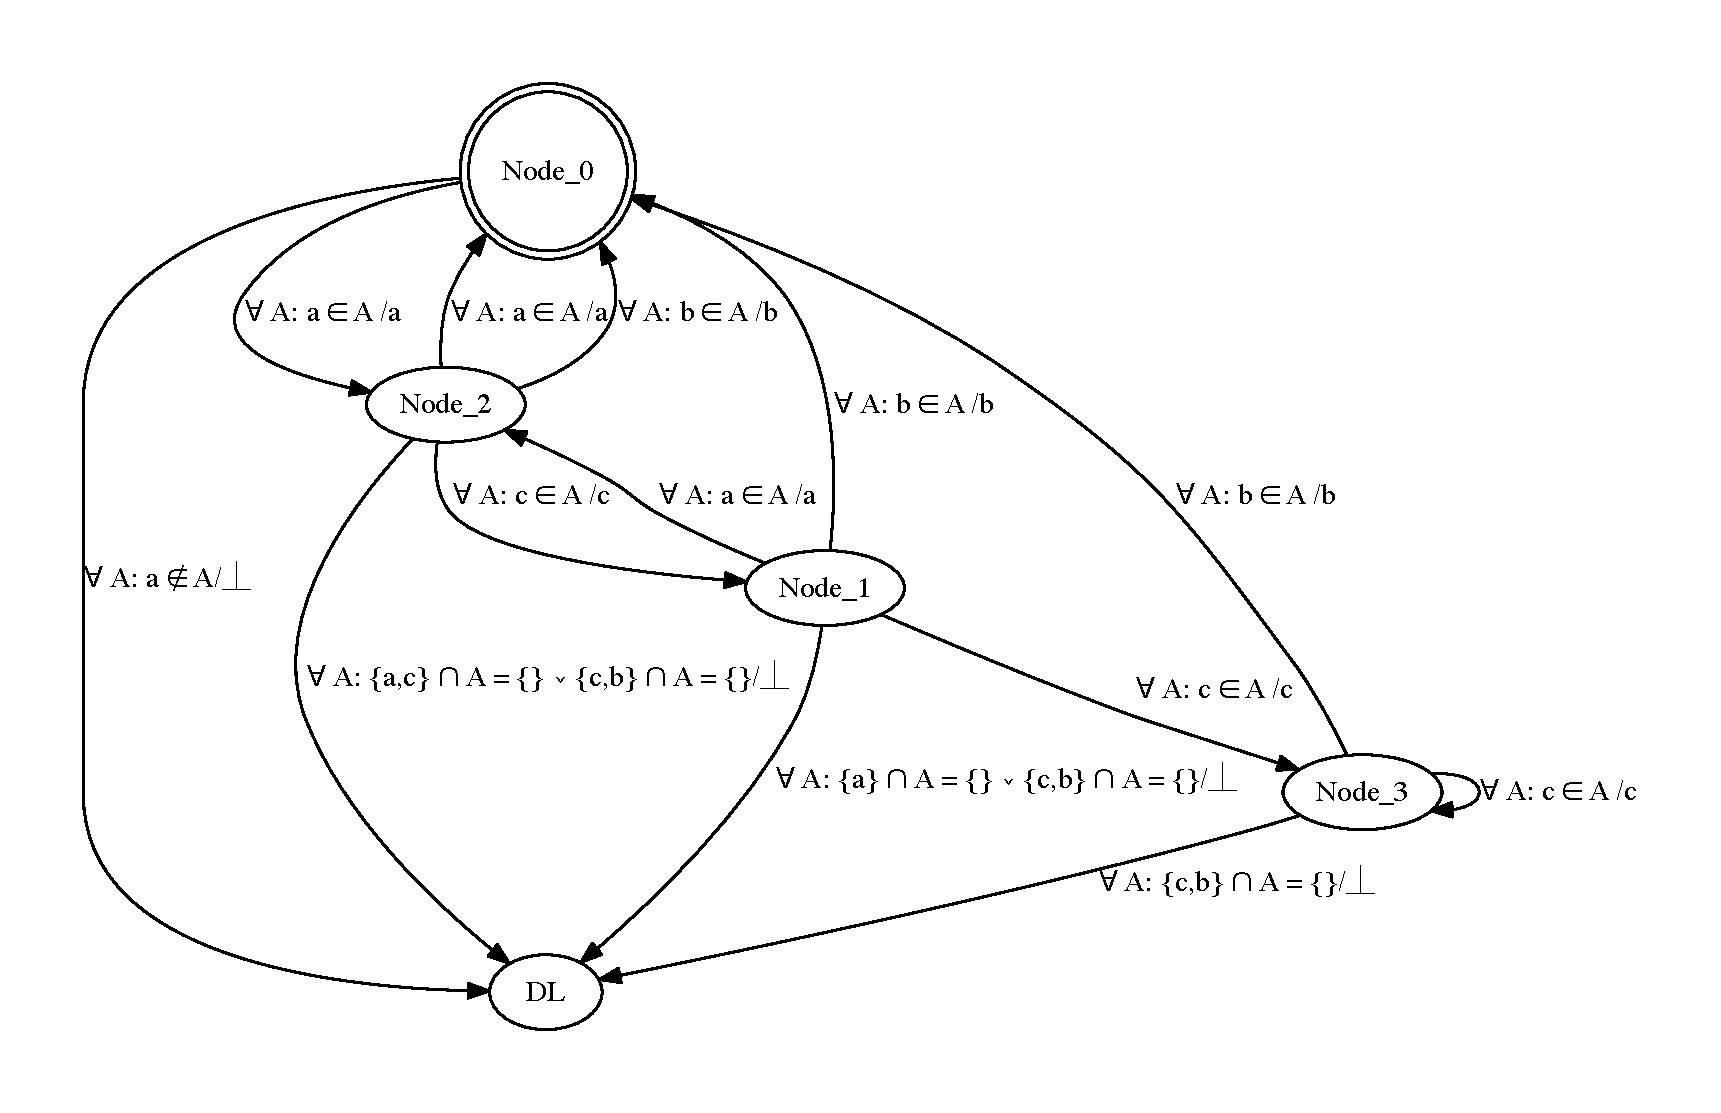
\includegraphics[width=\textwidth]{fsm0.pdf}
\end{center}
%%\vspace*{-10mm}
\caption{FSM resulting from applying the model map to CSP process $P$ from Example~\ref{ex:a}.}
 \label{fig:fsm0}
 \end{figure}
% ................................................................................... 

We are now in the position to state and prove the theorem about the model map 
fulfilling the satisfaction condition {\bf SC1} introduced in Section~\ref{sec:transltt}. To this end, we first introduce three lemmas.



\begin{lemma}\label{lemma:a}
Let $s\in \Sigma^*$ be any trace of $P$. Let $\underline n$ be the initial node of $G(P)$ and the initial state of $T(P)$. Let $n$ be the node of $G(P)$ denoting the process state $P/s$. Then for any input sequences $x\in \Sigma_I^*$ satisfying 
$\#x = \#s = k$   and $s(i)\in x(i)$, $\forall i\le k$, we have $x/s\in L(T(P))$ and $\underline n{\text{-after-}}x/s=n$. Furthermore,
for any $B\in \Sigma_I$, 
$$
B\in {\text{\rm Ref}}(P/s)\Leftrightarrow (x/s).(B/\bot) \in L(T(P))
$$
Conversely, any $x/s\in L(T(P))$ fulfils either
\begin{enumerate}
\item  $s\in {\text {\rm tr}}(P)$ and $s(i)\in x(i), \forall i\le \#(x/s)$,
or
\item $x/s=(x'.x_k)/(s'.\bot)$ with $s'\in {\text {\rm tr}}(P)$, $s(i)\in x(i), \forall i< \#(x/s)$ and $x_k\in {\text{\rm Ref}}(P/s')$. 
\end{enumerate}
\end{lemma}


The following lemmas are a direct consequence of Lemma~\ref{lemma:a}.


%----------------------------------------------------------------------------------
\begin{lemma}
For any $s\in \Sigma^*$, 
$$s\in {\text {\rm tr}}(P) \Leftrightarrow \exists x\in \Sigma_I^*: x/s \in L(T(P))$$
\end{lemma}
%-----------------------------------------------------------------------------

%--------------------------------------------------------------------------------
\begin{lemma}
For any $s\in \Sigma^*$ and $x_k\in \Sigma_I$, 
$$s\in {\text {\rm tr}}(P) \wedge  x_k\in {\text {\rm Ref}}(P/s)\Leftrightarrow \exists x\in \Sigma_I^*: x.x_k/s.\bot \in L(T(P))$$
\end{lemma}
%-------------------------------------------------------------------------------

\begin{theorem}
\label{th:sc1}
Consider the signature $Sig_1$ of CSP processes over fixed alphabet $\Sigma$ and the 
model map $T$ from CSP processes to finite state machines specified above.
Then the satisfaction condition {\bf SC1} is valid in the sense that
$$
\forall P, Q\in Sig_1: P \lessdet_F Q \Leftrightarrow   T(Q) \preceq T(P),
$$
where $\lessdet_F$ denotes failures refinement and $\preceq$ denotes reduction.
\end{theorem}
\begin{proof}
Applying the lemmas above, we can derive the following sequence of equivalence
transformations.
\begin{eqnarray*}
T(Q)\preceq T(P) &\Leftrightarrow & L(T(Q))\subseteq L(T(P))
\\ &\Leftrightarrow &
\forall x/s\in L(T(Q)):   x/s\in  L(T(P))
%%
\\ &\Leftrightarrow &  
\big(\forall x/s\in L(T(Q)): s\in\Sigma^* \Rightarrow x/s\in L(T(P)) \big) \wedge {}
\\ & & 
\big( \forall (x.x_k)/(s.\bot)\in L(T(Q)):  s\in\Sigma^* \Rightarrow 
(x.x_k)/(s.\bot)\in L(T(P)) \big)
%%
\\ &\Leftrightarrow &  
\big(\forall s\in\text{tr}(Q), x\in\{ z\in\Sigma_I^*~|~z/s\in L(T(Q)) \}:
\\ & & \tabc
s\in\text{tr}(P) \wedge x/s\in L(T(P))
\big) \wedge {}
\\ & & 
\big(\forall s\in\text{tr}(Q), x\in\{ z\in\Sigma_I^*~|~z/s\in L(T(Q)) \}, 
x_k\in\text{Ref}(Q/s):
\\ & & \tabc
s\in\text{tr}(P) \wedge x/s\in L(T(P)) \wedge x_k\in\text{Ref}(P/s)
\big)
%%
\\ &\Leftrightarrow &  
\big(\forall s\in\text{tr}(Q): s \in \text{tr}(P)\big) \wedge {}
\\ & & \big(\forall s\in\text{tr}(Q), x_k\in\text{Ref}(Q/s): 
s\in\text{tr}(P) \wedge x_k\in\text{Ref}(P/s)\big)
%%
\\ &\Leftrightarrow &  
\forall s\in {\text {\rm tr}}(Q):   s\in{\text {\rm tr}}(P) \wedge {\text {\rm Ref}}(Q/s)\subseteq {\text {\rm Ref}}(P/s)
%%
\\ &\Leftrightarrow & P \lessdet_F Q
\end{eqnarray*} 
\xbox
\end{proof}
 

% ==========================================================================
\subsection{A Test Case Map from Finite State Machines to CSP Processes}
\label{sec:tcmap}

% -------------------------------------------------------------------------
\subsubsection*{FSM Test Cases}

Following~\cite{DBLP:conf/hase/PetrenkoY14}, 
an \emph{adaptive FSM test case} 
$$
tc_\text{FSM}=(Q,\ii q,\Sigma_I,\Sigma_O,h,in)
$$ 
is a nondeterministic, observable, output-complete, acyclic FSM which only provides a single input in a given state. Running in FSM intersection mode with the SUT, the test case provides a specific input to the SUT; this input is determined by the current state of the test case. It accepts every output and transits either to a fail-state FAIL, if the output is wrong according to the test objectives, or to the next test state uniquely determined  by the processed input/output pair. Another state PASS indicates that
the test has been completed without failure. Both FAIL and PASS are termination states, that is, they do not have any outgoing transitions.

Since the test case state determines the input for all of its outgoing transitions, this input is typically used as a state label, and the outgoing transitions are just labelled by the possible outputs. A function $in : Q -\{  \text{PASS}, \text{FAIL} \} 
\fun\Sigma_I$ maps the states to these inputs. Termination states
of the FSM are not labelled with further inputs.

\begin{example}
Consider the FSM test case depicted in Fig.~\ref{fig:fsm0tc} which is specified
for the same input and output alphabets as defined for  the FSM presented in Example~\ref{ex:b}. The test case is passed by the FSM from Example~\ref{ex:b}, because 
intersecting the two state machines results in an FSM which always reaches the PASS state.
\xbox
\end{example}


% ...................................................................................
 \begin{figure}
 %%\hspace*{-40mm}
 \begin{center}
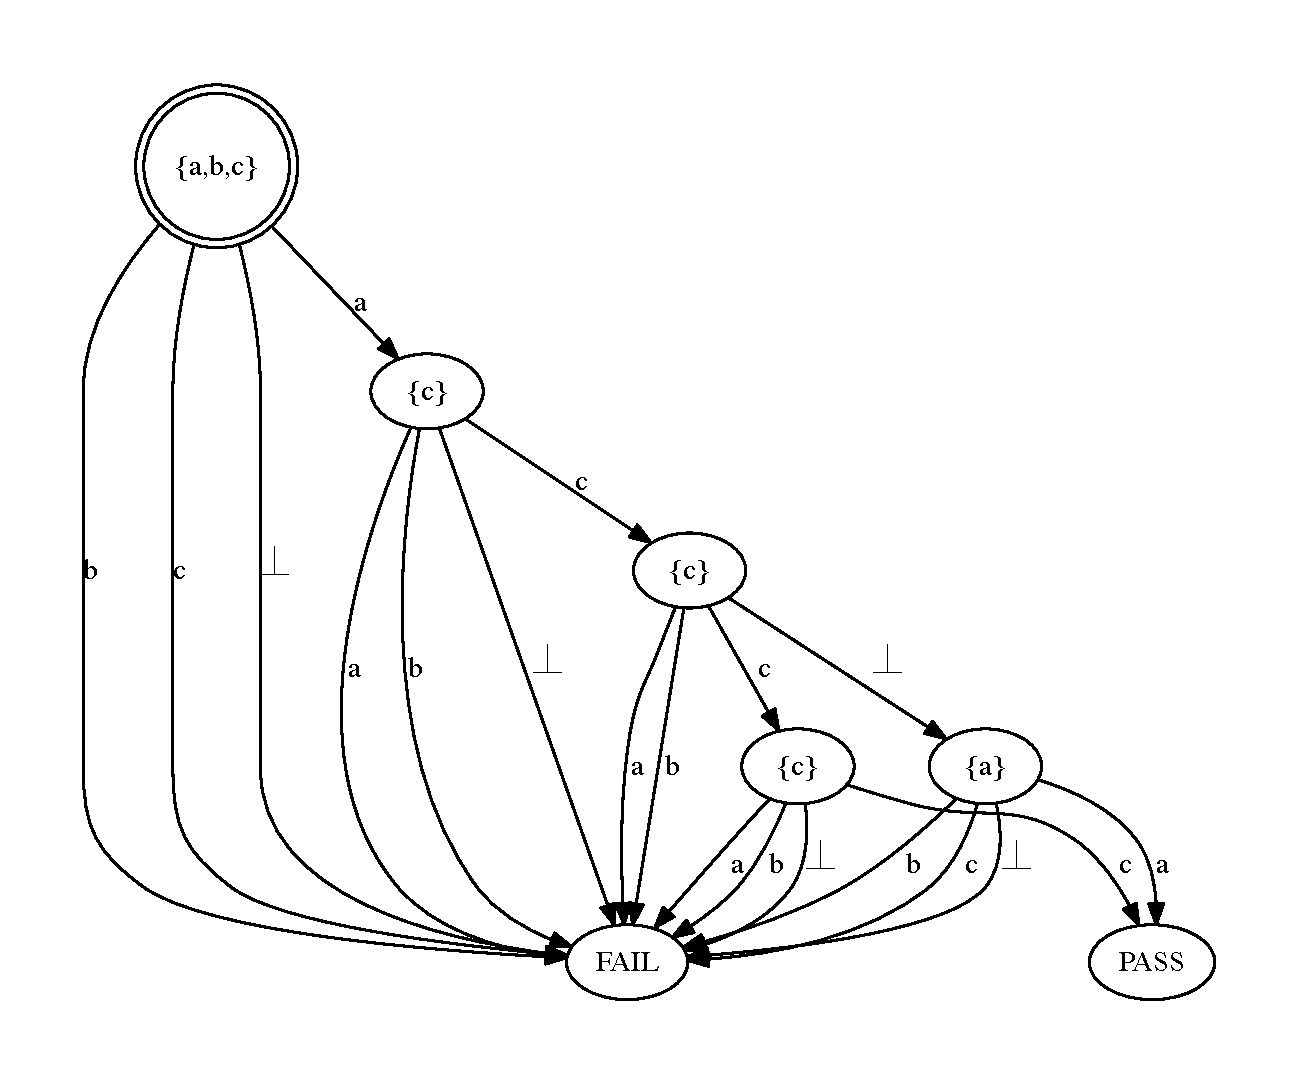
\includegraphics[width=.8\textwidth]{fsm0tc.pdf}
\end{center}
%%\vspace*{-10mm}
\caption{An FSM test case which is passed by the FSM presented in Example~\ref{ex:b}.}
 \label{fig:fsm0tc}
 \end{figure}
% ................................................................................... 

 


% -------------------------------------------------------------------------
\subsubsection*{CSP Test Cases}
A \emph{CSP test case} is a terminating process with alphabet 
$\Sigma\cup\{\dag,\bot,\tick \}$, where the extra events stand for 
(1) test  verdict FAIL ($\dag$), (2) timeout ($\bot$), and (3) test 
 verdict PASS ($\tick$). In principle, very general classes of CSP processes can be
 used for testing, as introduced, for example, in~\cite{peleska_testing_1996,peleska1997a}. For the purpose of this paper, however, we can restrict the possible variants of CSP test cases to the ones that are in the range of the test case map which is constructed next.



% -------------------------------------------------------------------------
\subsubsection*{Test Case Map}

The test case map $T^* :TC(FSM) \fun TC(CSP)$ is specified with respect to a fixed
CSP process alphabet $\Sigma$ extended by the events $\{\dag,\bot,\tick \}$ introduced
above
and the associated FSM input and output alphabets
$\Sigma_I = \power(\Sigma)-\{\varnothing\}$ and $\Sigma_O=\Sigma\cup \{\bot \}$.
Given an FSM test case $tc_\text{FSM}=(Q,\ii q,\Sigma_I,\Sigma_O,h,in)$, 
the image $T^*(tc_\text{FSM})$ is the CSP process $tc_\text{CSP}$ specified 
as follows.
\begin{eqnarray*}
tc_\text{CSP} & = & tc(\ii q)
\\
tc(q) & = & \big( e : \{ a\in in(q)\cup\{\bot\}~|~h_1(q,in(q),a)\notin \{\text{PASS},\text{FAIL}\} \} \bullet e \then tc(h_1(q,in(q),e) \big)
\\ & & \extchoice
\\ & & \big( e : \{ a\in in(q)\cup\{\bot\}~|~h_1(q,in(q),a) = \text{PASS} \} \bullet e \then \tick \then \Skip \big)
\\ & & \extchoice
\\ & & \big( e : \{ a\in in(q)\cup\{\bot\}~|~h_1(q,in(q),a) = \text{FAIL} \} \bullet e \then \dag \then \Skip \big)
\end{eqnarray*}


% ..........................................................................
\begin{example}
The FSM test case $tc_\text{FSM}$
shown in Fig.~\ref{fig:fsm0tc} is mapped by $T^*$ to the following
CSP test case.
\begin{eqnarray*}
T^*(tc_\text{FSM}) & = & P_1
\\
P_1 & = & \big(e:\{ b,c,\bot \} \bullet e \then \dag\then\Skip\big)
\extchoice
 \big( a \then P_2 \big) 
\\
P_2 & = & \big( e : \{ a,b,\bot \}\bullet e\then \dag\then\Skip  \big)
\extchoice
\big( c\then P_3 \big)
\\
P_3 & = & \big( e : \{ a,b \}\bullet e\then \dag\then\Skip  \big)
\extchoice
\big( \bot \then P_4 \big)
\extchoice
\big( c\then P_5 \big)
\\
P_4 & = & \big( e : \{ b,c,\bot \}\bullet e\then \dag\then\Skip  \big)
\extchoice
\big( a\then\tick\then \Skip \big)
\\
P_5 & = & \big( e : \{ a,b,\bot \}\bullet e\then \dag\then\Skip  \big)
\extchoice
\big( c\then\tick\then \Skip \big)
\end{eqnarray*}
\xbox
\end{example}

The following theorem shows the validity of the satisfaction condition {\bf SC2}
regarding the test case map, the model map, and the pass conditions for tests on CSP level and FSM level.

% ----------------------------------------------------------------------
\begin{theorem}
Fixing a CSP process alphabet $\Sigma$, the model map 
$T : \underline{Sig}_1 \fun FSM$ and the test case map $T^*:TC(FSM) \fun TC(CSP)$ fulfil satisfaction condition {\bf SC2} in the sense that
$$
\forall P\in \underline{Sig}_1, tc_\text{FSM}\in TC(FSM): T(P)\ \pass_2\ tc_\text{FSM} \Leftrightarrow
P\ \pass_1\ T^*(tc_\text{FSM})
$$
\end{theorem}
\begin{proof}
Let $T(P) = (Q,\ii q,\Sigma_I,\Sigma_O,h)$ and 
$tc_\text{FSM} = (Q',\ii q',\Sigma_I,\Sigma_O,h',in)$.

\noindent
We show by induction over the length of $s\in\Sigma_O^*$ that the following 
assertions hold for all $s$.
\begin{enumerate}
\item For every pass-trace $x/s \in L(T(P)) \cap L(tc_\text{FSM})$, 
there exists a pass-trace $u \in \text{tr}(P\parallel[\Sigma] T^*(tc_\text{FSM}))$, such that
$u\project\Sigma$ corresponds to $x/s$.

\item For every fail-trace  $x/s \in L(T(P)) \cap L(tc_\text{FSM})$, 
there exists a fail-trace trace 
$u \in \text{tr}(P\parallel[\Sigma] T^*(tc_\text{FSM}))$, such that
$u\project\Sigma$ corresponds to $x/s$.

\item For all $x/s\in L(T(P))$, 
the graph nodes of $G(P)$ and the states of $T(P)$ are related by
$$
\begin{array}{l}
G(P)/(s\project\Sigma) = \ii q\after (x/s).
\end{array}
$$

\item FSM test $tc_\text{FSM}$ and CSP test $T^*(tc_\text{FSM})$ perform consistent
state changes, in the sense that
$$
\begin{array}{l}
x/s\in L(T(P))\cap L(tc_\text{FSM}) \wedge  \ii q'\after (x/s) \not\in \{\text{PASS},\text{FAIL}\}
\Rightarrow {}
\\\tabd
T^*(tc_\text{FSM})/(s\project \Sigma) = tc(\ii q'\after (x/s)),
\end{array}
$$
where $tc(q)$ has been defined above with the test case map.

\end{enumerate}

Proof of 1 and 2 obviously proves the theorem; assertions~2 and 3 are 
needed to perform the induction argument.



For the base case, $s$ is the empty trace, so $x/s$ is empty as well. We have 
$G(P)/\varepsilon = \ii n = \ii q$, due to the definition of the model map. 
FSM test case $tc_\text{FSM}$ resides in its initial state $\ii q'$. By definition of the test case map above, $T^*(tc_\text{FSM})$ has initial CSP process state $tc(\ii q')$; this proves  Assertion~3 and Assertion~4 for the case $\#s = 0$. For assertions 1 and 2, there is nothing to
prove: no test can pass or fail on the empty trace.

For the induction hypothesis, assume that the four assertions have been proven for
$\#s \le k$ with $0\le k$.

For the induction step, assume that the FSM test has run through trace $x/s$ such that
$\#s \le k$ and $\ii q'\after (x/s) = q'$. The induction hypothesis gives us
$G(P)/(s\project\Sigma) = \ii q\after (x/s)$
from Assertion~3 and
$T^*(tc_\text{FSM})/(s\project \Sigma) = tc(q')$ from Assertion~4.
FSM test $tc_\text{FSM}$ will offer input $in(q')$ to the FSM $T(P)$ which is being tested. We make a case analysis for the outcomes of the resulting test step.

 

\noindent
{\bf Case~1.} $(x.in(q'))/(s.\bot) \in L(\ii q\after (x/s))$.\newline
By construction of $T(P)$, this is exactly the case if 
$in(q')\in r(G(P)/(s\project \Sigma))$. Since $tc_\text{FSM}$ is output complete,
$in(q')/\bot \in L(q')$. Depending on the nature of the test case, 
$q'\after (in(q')/\bot)$ is one of the deadlock states PASS, FAIL, or it is a
non-blocking FSM state, say, $q''$. Since $tc_\text{FSM}$ is observable, however, 
this post-state is uniquely determined. Observability of $tc_\text{FSM}$ 
implies further that the sets $\{ a\in in(q)\cup\{\bot\}~|~q\after(in(q)/a)\notin \{\text{PASS},\text{FAIL}\}$, $\{ a\in in(q)\cup\{\bot\}~|~q\after(in(q)/a) = \text{PASS} \}$, and $\{ a\in in(q)\cup\{\bot\}~|~q\after(in(q)/a) = \text{FAIL} \}$
used in the definition of $tc(q)$ are disjoint. As a consequence, $T^*(tc_\text{FSM})$
has exactly one choice to proceed and will come to the post-states that are analogous to those of $tc_\text{FSM}$: if $tc_\text{FSM}$ terminates in PASS(FAIL), then 
$T^*(tc_\text{FSM})$ will produced the events $\bot$ followed by 
$\tick(\dag)$ and terminate. If $tc_\text{FSM}$  transits to $q''$, CSP test case
$T^*(tc_\text{FSM})$ will perform $\dag$ as well and continue like process 
$tc(q'\after(in(q')/\bot)$

 

\noindent
{\bf Case~2.} FSM test $tc_\text{FSM}$ 
performs a transition into the FAIL-state. This
\xbox
\end{proof}

% ==========================================================================


